\documentclass[a4paper]{article}
\usepackage{amsmath, amsfonts, amssymb, amsthm}
\usepackage{booktabs}
\usepackage{color}
\usepackage{comment}
\usepackage{enumitem}
\usepackage[top=2cm,bottom=2cm,left=3cm,right=3cm]{geometry}
\usepackage{graphicx}
\usepackage{hyperref}
\usepackage{listings}
\usepackage{tikz}
\usepackage{url}
\usepackage{xspace}

%%% TIKZ
\usetikzlibrary{calc}
\usetikzlibrary{decorations}
\usetikzlibrary{positioning}
\usetikzlibrary{shapes}

%%% STYLE
\renewcommand{\familydefault}{\sfdefault}
\setlength\parindent{0pt}

%%% ENVIRONMENTS

% Question environment
\newtheoremstyle{que}% name
  {}% Space above, empty = `usual value'
  {}% Space below
  {}% Body font
  {}% Indent amount (empty = no indent, \parindent = para indent)
  {\bfseries}% Thm head font
  {}% Punctuation after thm head
  {\newline}% Space after thm head: \newline = linebreak
  {\thmname{#1}\thmnumber{ #2}:\thmnote{ #3}\vspace{\medskipamount}}% Thm head spec
\theoremstyle{que}
\newtheorem{question}{Question}

%%% MACROS

% Use to fix offset if an environment starts with an enumerate
\newcommand{\fixoffset}{\mbox{}\vspace*{-\bigskipamount}\vspace*{-\medskipamount}}
\newcommand{\eg}{{\em e.g.}\xspace}
\newcommand{\ie}{{\em i.e.}\xspace}
\mathchardef\mhyphen="2D
\newcommand\points[1]{%
\ifnum1<0#1\relax%
    {\bf \small [#1~marks]}%
  \else%
    {\bf \small [#1~mark]}%
  \fi%
}%

\newcommand{\module}{COMP0143: Cryptocurrencies}
\newcommand{\university}{University College London}
\newcommand{\assessment}{Coursework}
\newcommand{\releaseDate}{November 8, 2024}
\newcommand{\dueDate}{December 11, 2024 at 16:00 UK time}
\newcommand{\feedbackDate}{TBD}
\newcommand{\weight}{40\%}
\newcommand{\pointsTotal}{100 marks}

\begin{document}

\title{\module\\[0.25cm]\assessment}
\author{\university}
\date{Released: \releaseDate\\[0.25cm]Due: \dueDate}
\maketitle

\newpage

%%%%%%%%%%%%%%%%%%%%%%%%%%%%%%%%%%%%%%%%%%%%%%%%%

\begin{question}[\points{25}]
  \fixoffset
  \begin{enumerate}[label=(\alph*)]
    \item 
    \item[(i)] To compute \( C \), we first hash our leaves, the elements of \( S \), to get \( H_1, \ldots, H_9 \). We can then compute the internal nodes \( H_{10}, H_{11}, H_{12} \) as follows:
\[
H_{10} = \text{H}(H_1 || H_2 || H_3)
\]
\[
H_{11} = \text{H}(H_4 || H_5 || H_6)
\]
\[
H_{12} = \text{H}(H_7 || H_8 || H_9)
\]
Finally, \( C \) can be calculated as:
\[
C = H_{13} = \text{H}(H_{10} || H_{11} || H_{12})
\]
A figure \ref{fig:merkle_tree} shows the full Merkle Tree.
\begin{figure}[h!]
    \centering
    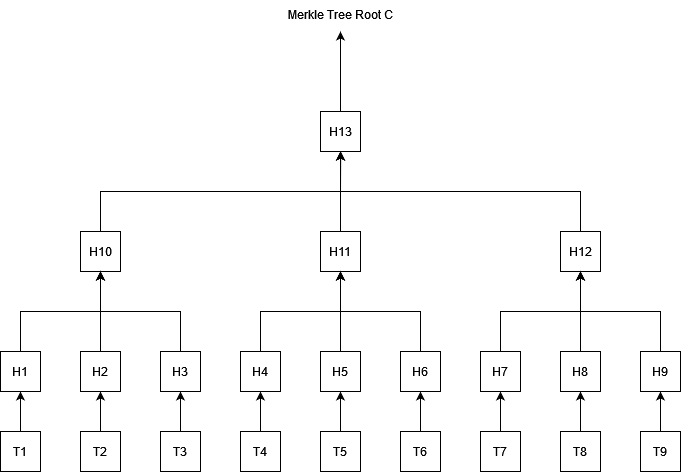
\includegraphics[width=0.5\textwidth]{Merkle Tree example.drawio.png} % Adjust the width as needed
    \caption{Merkle Tree Structure}
    \label{fig:merkle_tree}
To prove \( t_4 \) is in \( S \) we can compute the Merkle Proof as follows:
\[
C = \text{H}(H_{10}||\text{H}(\text{H}(t_4)||H_5||H_6)||H_{12})
\]

\end{figure}
    \item[(ii)] 
    \item ...
  \end{enumerate}
\end{question}

\newpage

%%%%%%%%%%%%%%%%%%%%%%%%%%%%%%%%%%%%%%%%%%%%%%%%%

\begin{question}[\points{25}]
  \fixoffset
  \begin{enumerate}[label=(\alph*)]
    \item Add your answers here.
    \item ...
  \end{enumerate}
\end{question}

\newpage

%%%%%%%%%%%%%%%%%%%%%%%%%%%%%%%%%%%%%%%%%%%%%%%%%

\begin{question}[\points{30}]
  \fixoffset
  \begin{enumerate}[label=(\alph*)]
    \item Add your answers here.
    \item ...
  \end{enumerate}
\end{question}

\newpage

%%%%%%%%%%%%%%%%%%%%%%%%%%%%%%%%%%%%%%%%%%%%%%%%%

\begin{question}[\points{20}]
  As your solution, please submit the completed {\tt TicTacToe.sol} file.
\end{question}

\newpage

\end{document}
